\chapter{Rinnovo}
\section{Vecchio cabinato}
Il vecchio cabinato è rimasto fermo per oltre venti anni. Quando è stato collegato per la prima volta alla corrente elettrica dopo questo lungo periodo di tempo purtroppo non c’è stato quasi alcun accenno di funzionamento. L’unico segno di vita che ha dato è stato un flash rapido sullo schermo all’accensione della macchina. Molto probabilmente il malfunzionamento è stato favorito dal clima umido in cui è stato collocato il cabinato per tutto il tempo in cui non è stato in funzione. È possibile evincere la sua vecchia funzione grazie al numero, la disposizione e il nome dei bottoni sulla plancia. Erano presenti cinque tasti gialli centrali con sopra stampata la scritta “HOLD”. Sopra ognuno, era integrata anche una scritta di “STOP”. Sulla destra c’era il normalissimo pulsante verde di “START” mentre sulla sinistra c’era un pulsante rosso con sopra scritto “RISK GETTONI”. Data la presenza di un distributore di ticket, il cabinato poteva assumere la funzione di Slot Machine, anche se è sicuramente nato per supportare nel pieno delle sue funzionalità qualsiasi video poker. La macchina era composta da:
\begin{itemize}
\item Monitor\\
Lo schermo del vecchio cabinato era un tubo catodico. I due grandi produttori di monitor per macchina da sale giochi sono state Hantarex e Fenice. Lo schermo del cabinet era un Hantarex che è stato necessario sostituire, sia per semplificare il collegamento con il nuovo PC, sia perché col tempo aveva riportato fin troppi deterioramenti. Inoltre la vista di un possibile giocatore ne risentirebbe molto meno con un monitor LCD.
\item Gettoniera \\
Il funzionamento di una gettoniera non è affatto complesso. Al passaggio e al riconoscimento del gettone viene aggiunto un credito, proprio come se venisse premuto un bottone.
\item Distributore di ticket \\
A gioco terminato può capitare che il videopoker debba pagare il giocatore. Questo può avvenire tramite due strade: restituendo altri gettoni, cambiabili alla casa per soldi veri, o pagando in ticket. I ticket sono molto più versatili dato che è anche possibile renderli delle vere e proprie valute, scambiabili per premi che offre la sala giochi.
\item Motherboard \\
La scheda sfruttava lo standard \gls{jamma}, diventato obsoleto a causa delle limitazioni di input e output rispetto a sistemi di gioco sempre più evoluti. Le schede madri dei cabinati arcade moderni utilizzano uscite video/audio più moderne (VGA, Jack da 3,5mm ecc.)
\item Gioco \\
I vecchi videogiochi venivano montati sulla scheda madre tramite delle cartucce contenenti, appunto, il gioco. Questo semplice meccanismo rendeva anche possibile cambiare gioco o macchina in qualsiasi momento.
\item Speaker \\
È stato necessario anche cambiare gli speaker, sia perché vecchi, sia perché erano mono e non stereo. Il connettore inoltre seguiva lo standard JAMMA e non era quindi compatibile con il nuovo sistema.
\end{itemize}
 \section{Restauro}
Il restauro è stato un lavoro lungo e dispendioso, anche in termini economici. Acquistare un cabinato completamente nuovo è sempre comunque molto più costoso e limitativo di un rinnovo. Questo perché per sistemare una vecchia macchina il costo dipende soprattutto dai soli materiali necessari o mancanti. L’acquisto di una macchina preassemblata invece prevede le compere di tutti i pezzi, il montaggio, la spedizione ecc.\\Per la realizzazione del cabinato gli unici costi gravosi affrontati sono stati:
\begin{itemize}
\item L’acquisto di tutti i componenti facenti parte della plancia (Bottoni e Joystick) e della scheda di encoding.\\
\item L’acquisto di vernici per metallo e legno.\\
\item L’acquisto e la lavorazione di due pezzi in legno e di uno in plexiglass.\\
\end{itemize}
 I pezzi acquistati comprendono sedici pulsanti di diverso colore (Figura~\ref{fig:chrome}), sei blu, sei rossi, due bianchi e due verdi. I due pulsanti verdi hanno inoltre un disegno riportante il numero di giocatori (uno o due).\\
\begin{figure}[!ht]
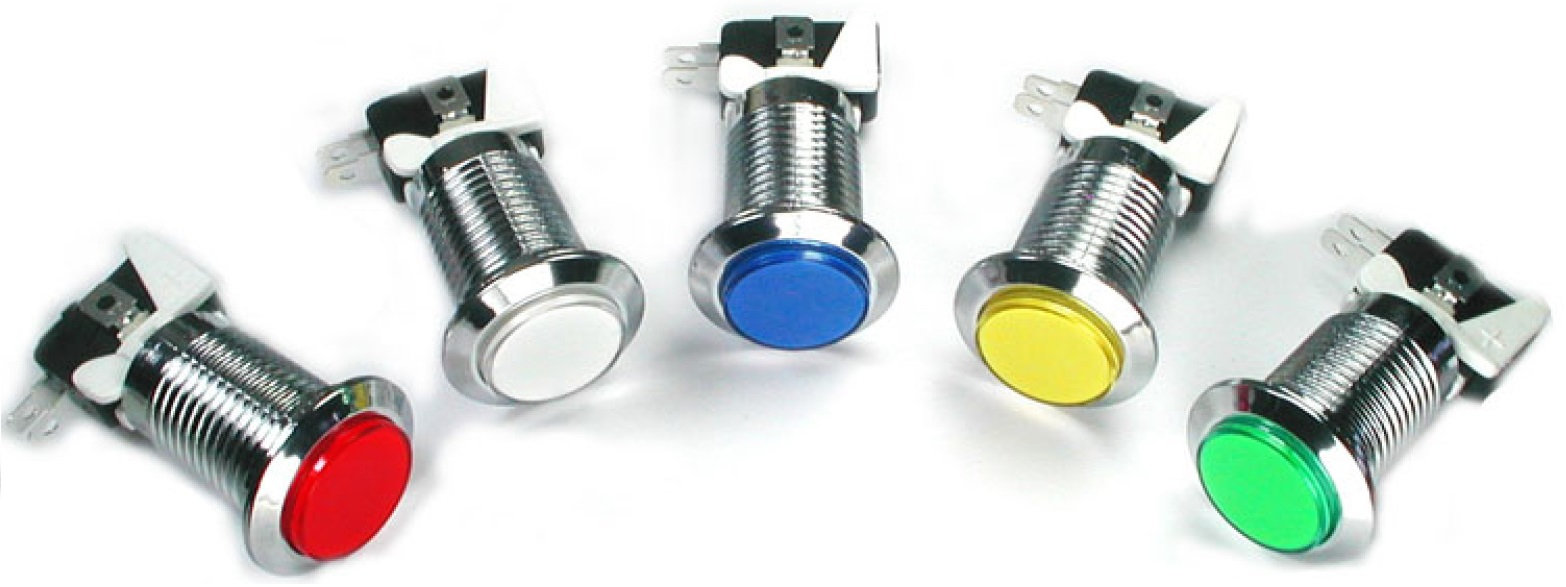
\includegraphics[scale=0.16]{chrome}
\centering
\caption{Esempi di pulsanti}
\label{fig:chrome}
\end{figure}
\\ I pulsanti bianchi sono i pulsanti per aggiungere i crediti, necessari in quanto la gettoniera è stata rimossa per rendere il gioco gratuito. I dodici pulsanti blu e rossi infine sono i normali tasti  destinati al gioco, sei per il primo giocatore e sei per il secondo. Non tutti i videogiochi in realtà richiedono sei pulsanti a testa per essere giocati. Dato che sulla macchina verrà installato un software di emulazione console sarà possibile scegliere tra diversi tipi di emulatori. Un controller del Neo Geo per esempio, possiede di fatto solo quattro tasti. Di conseguenza non esistono giochi che nativamente richiedono più di quattro tasti per quel tipo di console. Esistono anche videogiochi che richiedono addirittura fino a otto tasti per essere giocati ma la mancanza di spazio sulla plancia non ha permesso l’inserimento di ulteriori tasti oltre ai dodici già presenti. Inoltre, giochi con questo prerequisito sono molto rari, spesso poco popolari o comunque meno frequenti dei grandi classici in cui a volte basta anche solo un pulsante (come \textit{Pac-Man}).
\begin{figure}[!ht]
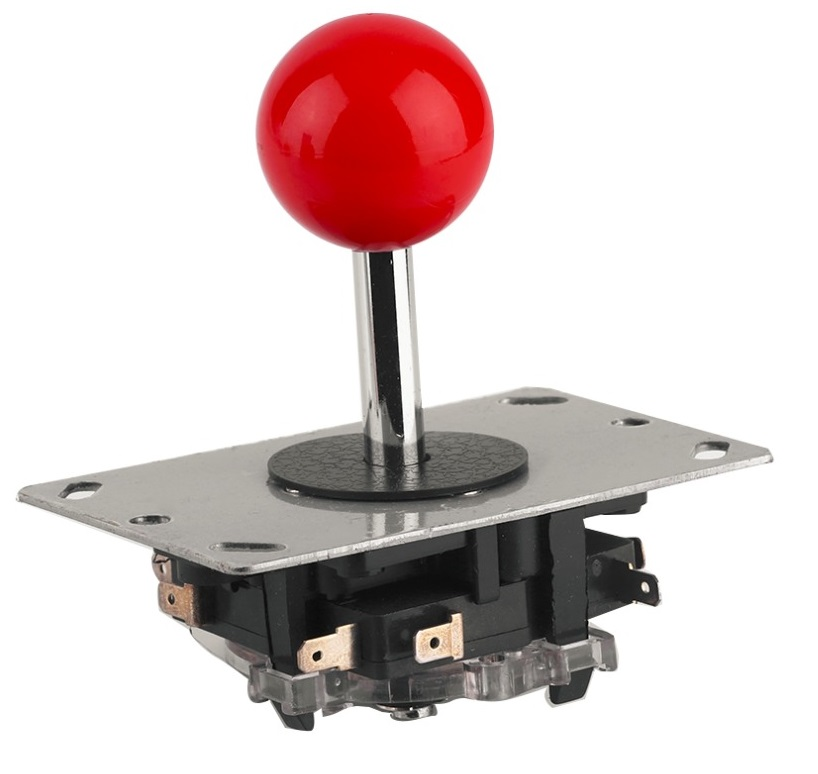
\includegraphics[scale=2.1]{sanwa}
\centering
\caption{Joystick usato per il restauro}
\label{fig:sanwa}
\end{figure}
\\Altri due pezzi fondamentali sono i joystick (Figura~\ref{fig:sanwa}). Il joystick è l’apparecchio a forma di leva che, sostanzialmente, riconosce i movimenti. I movimenti standard normalmente sono su, giù, destra, sinistra ma esistono anche joystick che permettono una maggiore precisione a otto direzioni o altri limitativi che ne permettono solo due. Sui Joystick del cabinato è possibile arrivare fino a otto direzioni, ma è possibile limitare i movimenti grazie ad un Restrictor Gate.\\
L’ultimo pezzo fondamentale è la scheda per l’encoding dei tasti. Il componente verrà approfondito nell’apposito capitolo.\\I pezzi in metallo arrugginiti sono stati carteggiati e ridipinti. Alcuni pezzi in legno erano malmessi o non erano adatti al progetto finale ed è stato necessario fabbricarne di nuovi. Questa operazione è stata necessaria per la plancia, che non aveva ovviamente il layout adatto all’inserimento dei nuovi componenti, e per la parte anteriore in cui prima risiedeva la gettoniera.\\Tutte le vecchie viti arrugginite sono state sostituite con delle nuove. Anche i due lucchetti sono stati cambiati in quanto malmessi. Inoltre è stata aggiunta una striscia di LED multicolore RGB su una buona parte dei bordi del mobile. Per disporla meglio, è stata fatta passare attraverso dei nuovi fori, praticati appositamente per permettere il passaggio di essa. La tonalità del colore è modificabile tramite un telecomando. Dato che quest’ultimo funziona ad infrarossi, è stato necessario piazzare il relativo sensore in un luogo nascosto ma comunque raggiungibile. È stato quindi posizionato all’interno dello sportello soprastante al punto in cui c'è la multipresa, per evitare l’uso di ulteriori prolunghe.\\All’interno del cabinet è stato inserito un personal computer. Per emulare videogiochi datati non è necessario un hardware particolarmente nuovo, infatti è stato impiegato un PC usato e ormai vecchio che tra l’altro era molto impolverato. Le specifiche tecniche sono le seguenti:\\
Scheda madre : Asus M3A\\
Processore: AMD Phenom 9750 Quad-Core Processor 2.4 GHz\\
Memoria RAM: Samsung 512MB Ram DDR2\\
Hard Disk: 40 GB HDD Maxtor DiamondMax Plus 8 ATA/133 IDE\\
Scheda Video: GeForce 8400 GS (Nvidia G86)
